\chapter{System implementation with Robot controller module}
\indent This chapter describes how all of components mentioned above are assembled. In design, I apply top-down approach in system development process. First, system is broken down into modules in which each system's function is handled separately. Next, functions of modules are presented in groups of communicating interfaces and groups of internal processing methods. Consequently, modules is divided into smaller and more dedicated units.

For each module, design pattern is engaged correspondingly to its operation behavior for the sake of ease in maintenance and convenience for extensibility.

Finally, when the system walking through all unit test cases, it is connected with the Delta robot to accomplish desired activities.

\section{System implementation}
\subsection{Whole system class diagram}
Figure \ref{fig:class_diagram} mentions all system ``workers'' known as classes \footnote{For convenient mentioning, interfaces are included}. These classes are organized in hierarchy and has relationship with each other. Some are compositions. Some are inheritances. Some have references to another classes. The detail of class relationships will be explained in upcoming sections.

    \begin{figure}[H]
		\centering
		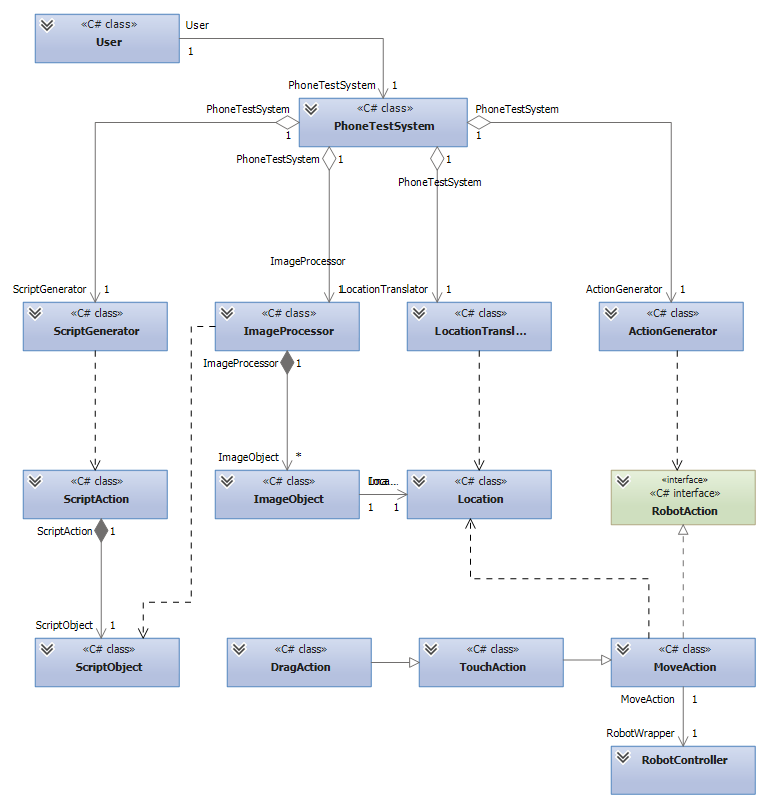
\includegraphics[scale=0.75]{Chapters/Fig/class_diagram.png}
		\caption{System class diagram}
		\label{fig:class_diagram}
	\end{figure}

\subsection{Main components of the system}
System consists of 3 main modules, which are Image Processing module, Script Managing module and Robot Action Handling module. Image Processing module involves in detecting and recognizing screen elements along with managing and organizing them for further access. Script Managing module does the job of operating test cases. Robot Handling module defines the movements of the robot and proposes inducing methods to other components so as to have the robot working.

	\begin{figure}[H]
		\centering
		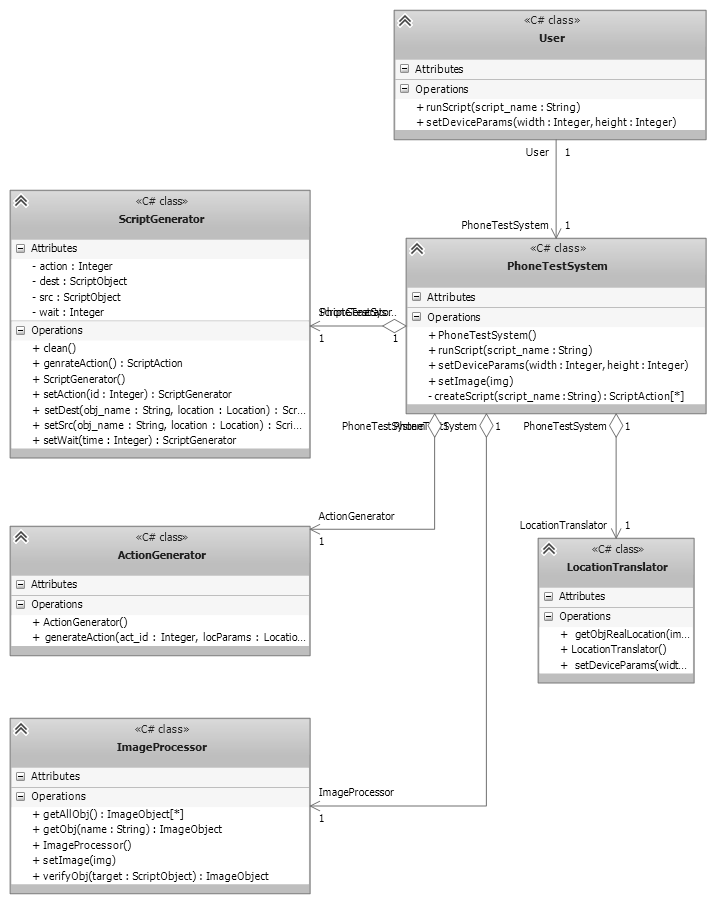
\includegraphics[scale=0.75]{Chapters/Fig/main_class.png}
		\caption{System main components}
		\label{fig:main_class}
	\end{figure}

There are also some assisting classes. PhoneTestSystem takes responsibility for wrapping up all modules and provide interface functions to user. LocationTranslator holds user input parameters with the purpose of converting actual phone screen location into pixel location in screen image and vice versa.

\subsection{Image Processor structure}

	\begin{figure}[H]
		\centering
		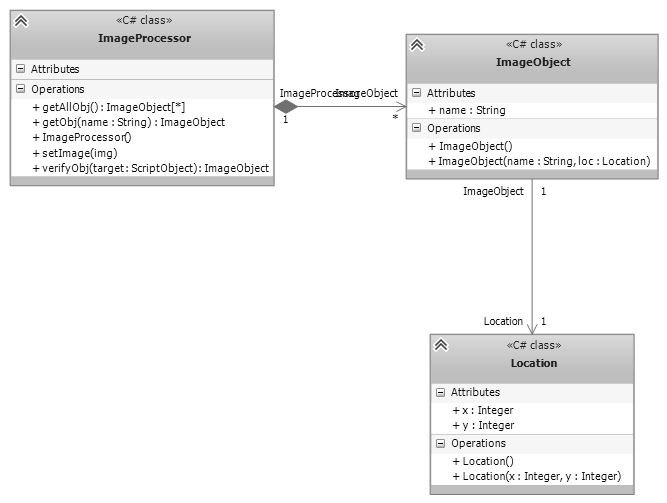
\includegraphics[scale=0.75]{Chapters/Fig/img_processor.png}
		\caption{Image Processor structure}
		\label{fig:img_processor}
	\end{figure}

\subsection{Script Generator structure}

	\begin{figure}[H]
		\centering
		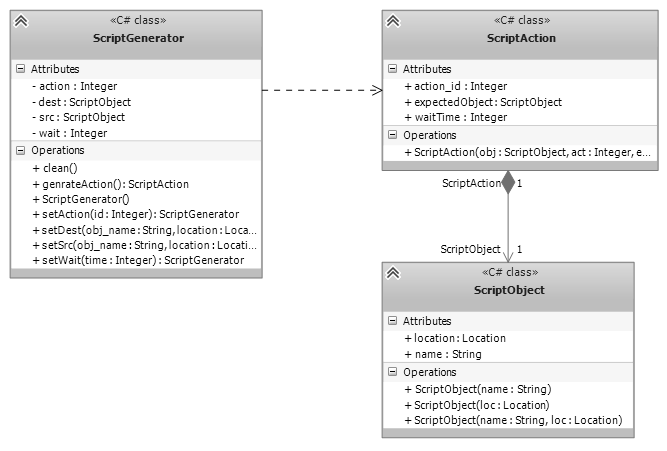
\includegraphics[scale=0.75]{Chapters/Fig/script_gen.png}
		\caption{Script Generator structure}
		\label{fig:script_gen}
	\end{figure}

\subsection{Action Generator structure}

	\begin{figure}[H]
		\centering
		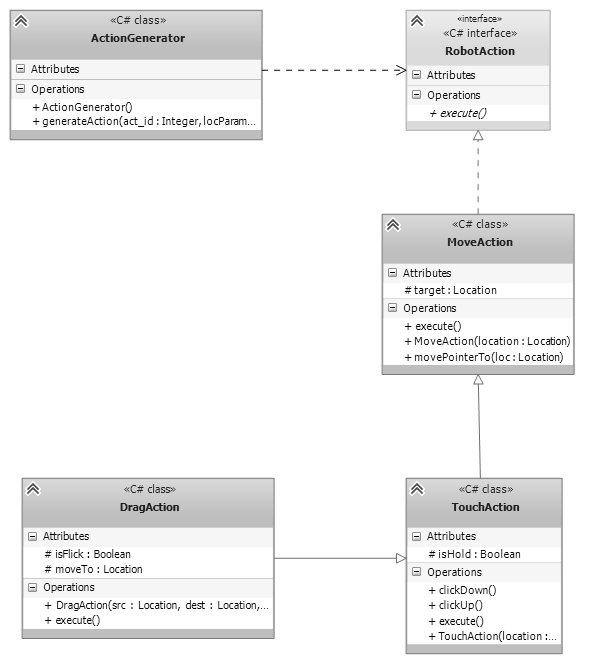
\includegraphics[scale=0.75]{Chapters/Fig/act_gen.png}
		\caption{Action Generator structure}
		\label{fig:act_gen}
	\end{figure}

\section{Robot interface command}

	\begin{itemize}
		\item[--] GotoXYZ
		\item[--] MoveToDest
		\item[--] ClickUp
		\item[--] ClickDown
	\end{itemize}
